\makeatletter
\newcommand*{\textoverline}[1]{$\overline{\hbox{#1}}\m@th$}
\makeatother

\subsection{Digital front end}\label{sec:frontend}
The digital front end (DFE) consist of three parts, D flip-flop with a NAND gate and a NOR gate. This can been seen in Fig.~\ref{fig:Global_schematic_DFE_figure}. The D flip-flop synchronizes the incoming data and the NAND/NOR gates mixes the signal with the local oscillator in the digital domain. The DFE works in a high frequency domain and it needs to switch fast; therefore thin oxide transistors are used. The drawback of this kind of transistors is that they allow a low maximum Vds (max 1.2V), that limits the maximum output power. To solve this problem a level shifter is used to increase the power at the output stage. The level shifter is discussed in section ~\ref{sec:levelshifter}. 

\begin{figure}[h]
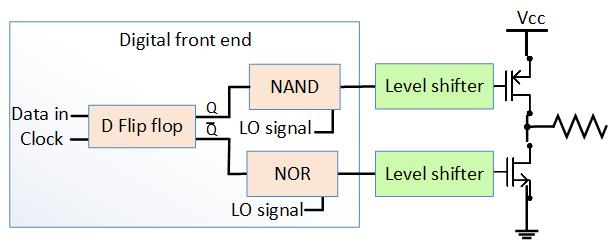
\includegraphics[width=0.5\textwidth]{Global_schematic_DFE.jpg}
\caption{One side of the diagram of the new digital front end.}
\label{fig:Global_schematic_DFE_figure}
\end{figure}

\subsubsection{D flip-flop}\label{sec:frontend}
The two main technologies to create a flip flop are CMOS and CML. CMOS is relatively less complex in comparison to CML, therefore it covers less space. The main advantage for CML design is that the complex structure gives more degrees of freedom to tune the output. In this project the CMOS design is used, because it is less complex, single-ended and it can be realised in a short time period.There are a couple of challenges when designing a D flip-flop, for example the operation speed and the transition time of the output at the rising clock.

The CMOS D flip-flop shown on page 2 in~\cite{powerdac} and page 17 in~\cite{coursebook} is used as starting point in the project. The schematic of their circuit is shown in Appendix A, Fig.~\ref{fig:D_flip_flop_ previous_group_figure}. The schematic of the new, improved, circuit consists of 32 transistors and is showed in Fig.~\ref{fig:D_flip_flop_schematic_figure}. There are three changes made in comparison with the old schematic to improve the synchronization. The first change is that a second output has been added to flip-flop, to reduce the amount of flip-flops. The second change holds an addition NMOS transitor that is used as a switch and the last change is related to different transistor sizes, to reduce output delay.
\begin{figure}[h]
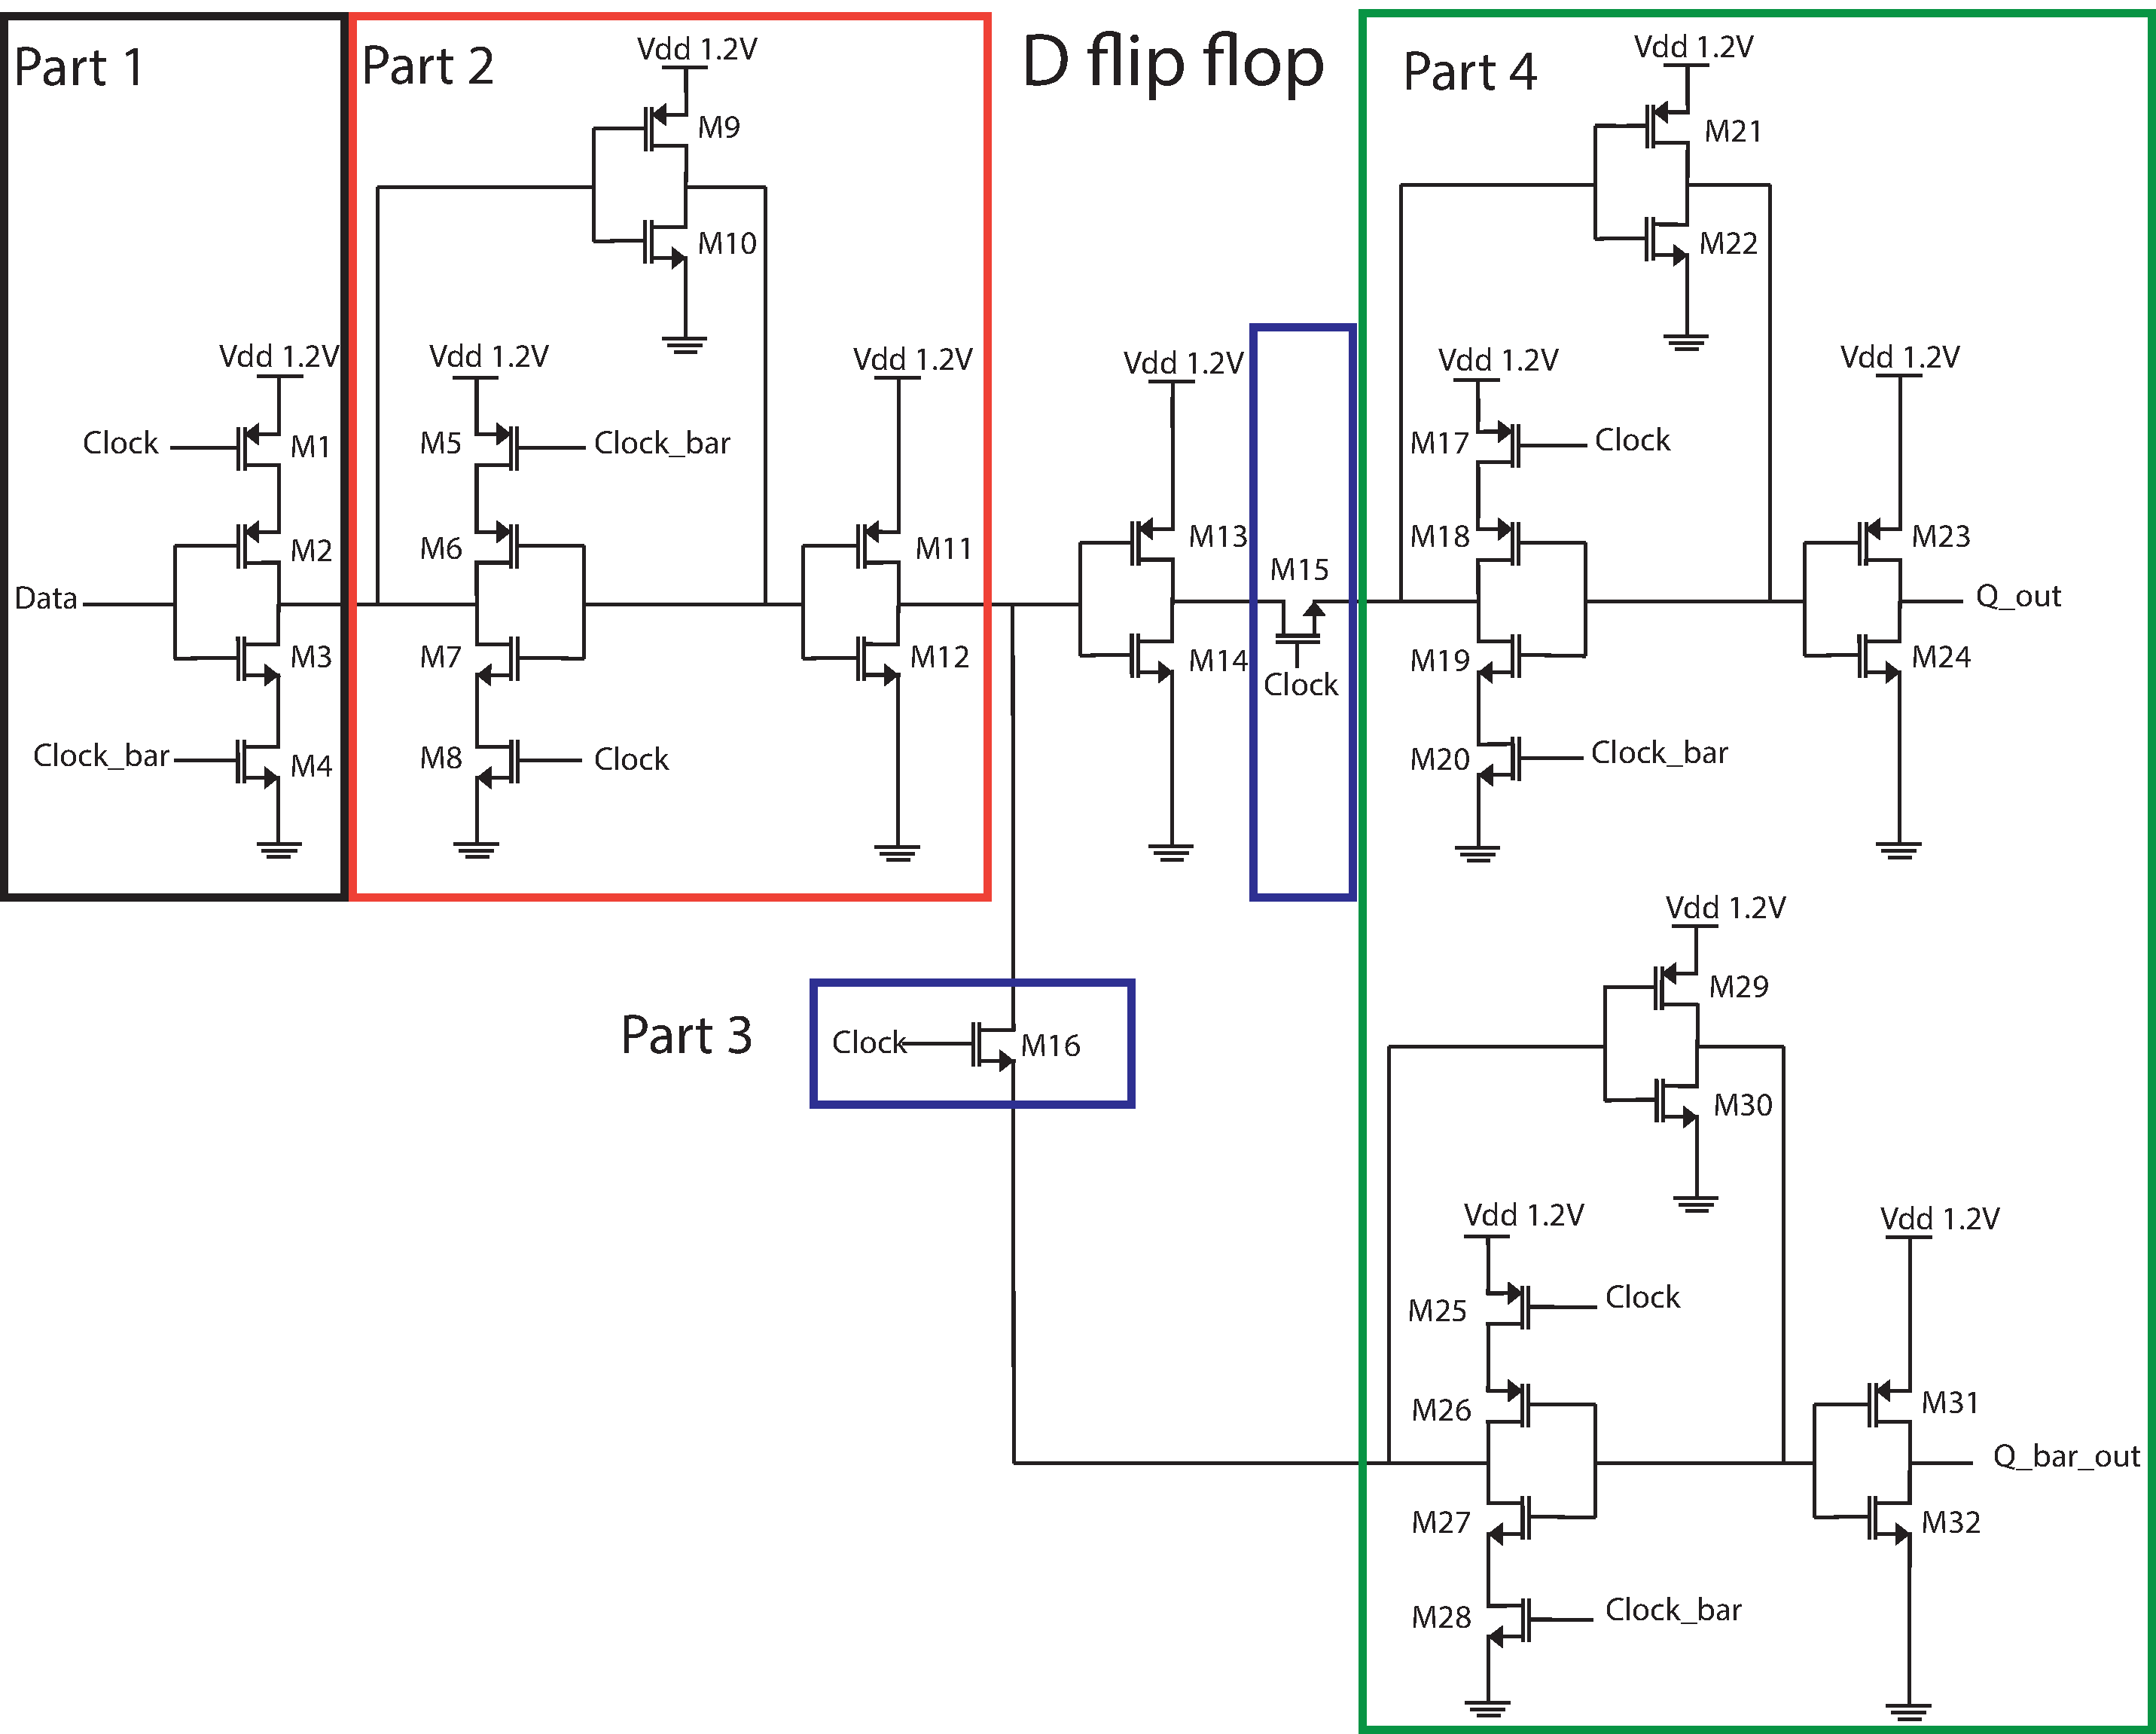
\includegraphics[width=0.5\textwidth]{D_flip_flop_new_schematic.pdf}
\caption{The improved D flip-flop schematic.}
\label{fig:D_flip_flop_schematic_figure}
\end{figure}

To explain the principle of a master-slave D flip-flop, the schematic can be divided into four parts,the settle time of the data, master latch, two switches and slave latch. In the first part, the data will be set when the clock is low. The second part, the master will follow the signal of the first part when the clock is low and hold the data when the clock is high. In the third part, the switches will be closed when the clock is high and the slave latch, which is part four, sets the data. When the clock is low the NMOS transistor in part three is open en the slave latch holds the data. 
The size of the PMOS and NMOS transistors in the master latch, slave latch and settling of the data are the same. The size of the NMOS transistor is set on 50nm x 90nm (length x width). The length of the PMOS transistor is the same, but the width of the PMOS transistor is determined with a parameter sweep to get the smallest delay of transition. In the parameter sweep the clock frequency is set to 1 GHz and the data frequency is set to 500 MHz. The results are shown in the Appendix A, Fig.~\ref{fig:parametersweep_changing_w_high_to_low_figure} and \ref{fig:parametersweep_changing_w_low_to_high_figure}. The optimal width of the PMOS transistor is 120nm, because it gives the smallest transition delay. The ratio of the widths of the PMOS and NMOS transistors is 1.33:1. (Wp:Wn)

The sizes of the switching NMOS transistors (part 3, transistor M16 and M15) are also determined with a parameter sweep with the same settings. The results are shown in Appendix A Fig.~\ref{fig:Parameter_sweep_changing_w_of_the_swiching_nmos_high_to_low_figure} and~\ref{fig:Parameter_sweep_changing_w_of_the_swiching_nmos_low_to_high_figure} in Appendix A. The optimal value of the width is 280nm. A comparison is made with the results of this value and the D flip-flop schematic of~\cite{powerdac}. The result is shown in Fig.~\ref{fig:Comparison_old_schematic_and_new_schematic_high_figure} and~\ref{fig:Comparison_old_schematic_and_new_schematic_low_figure}. The overall delay of the rise and fall time is reduced with 12ps to 13ps of Q and \textoverline{Q}, but at the cost of 2ps in the transition from low tow high of \textoverline{Q}. 

\begin{figure}[h]
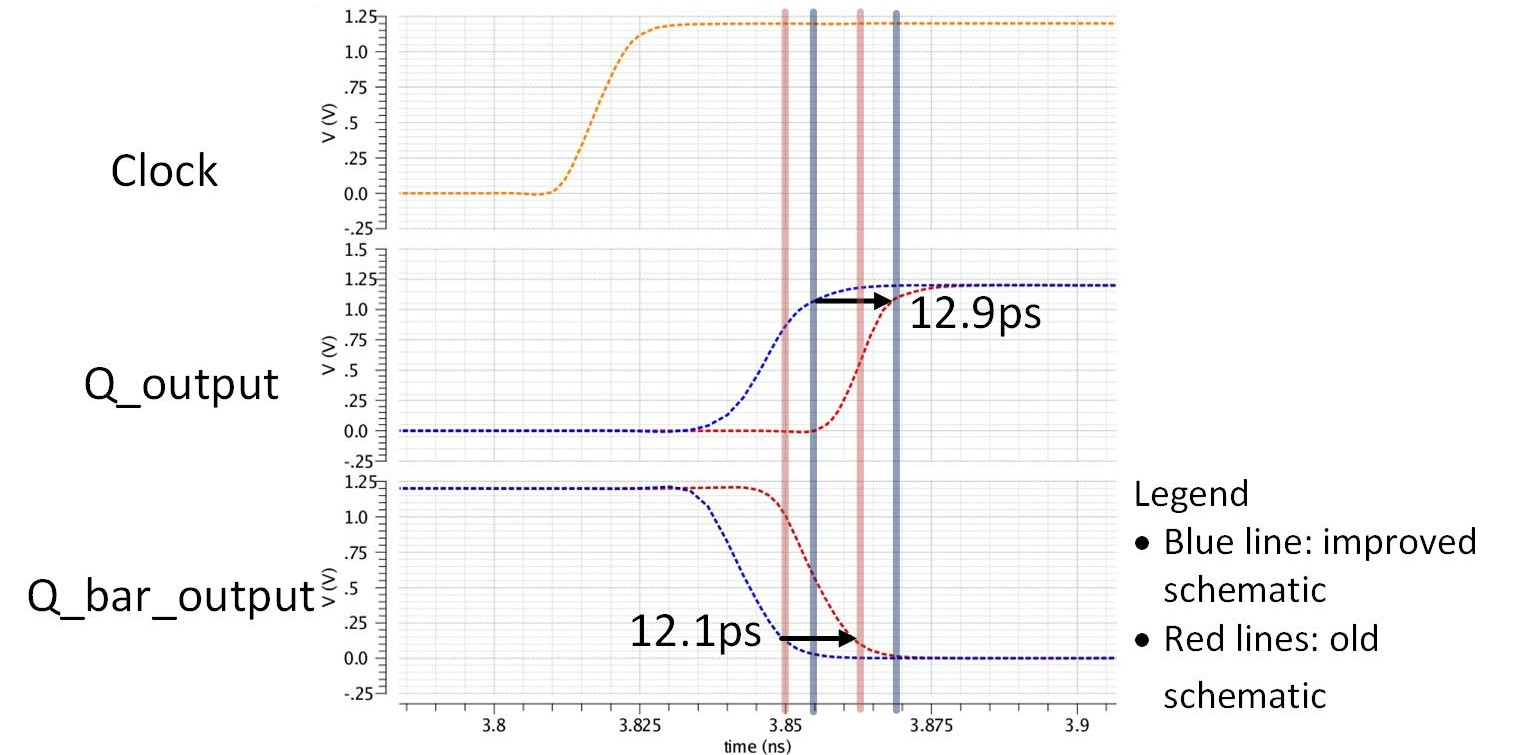
\includegraphics[width=0.5\textwidth]{Comparison_old_schematic_and_new_schematic_high.jpg}
\caption{Comparison of the transition delay before and after improvements when the data is high }
\label{fig:Comparison_old_schematic_and_new_schematic_high_figure}
\end{figure}

\begin{figure}[h]
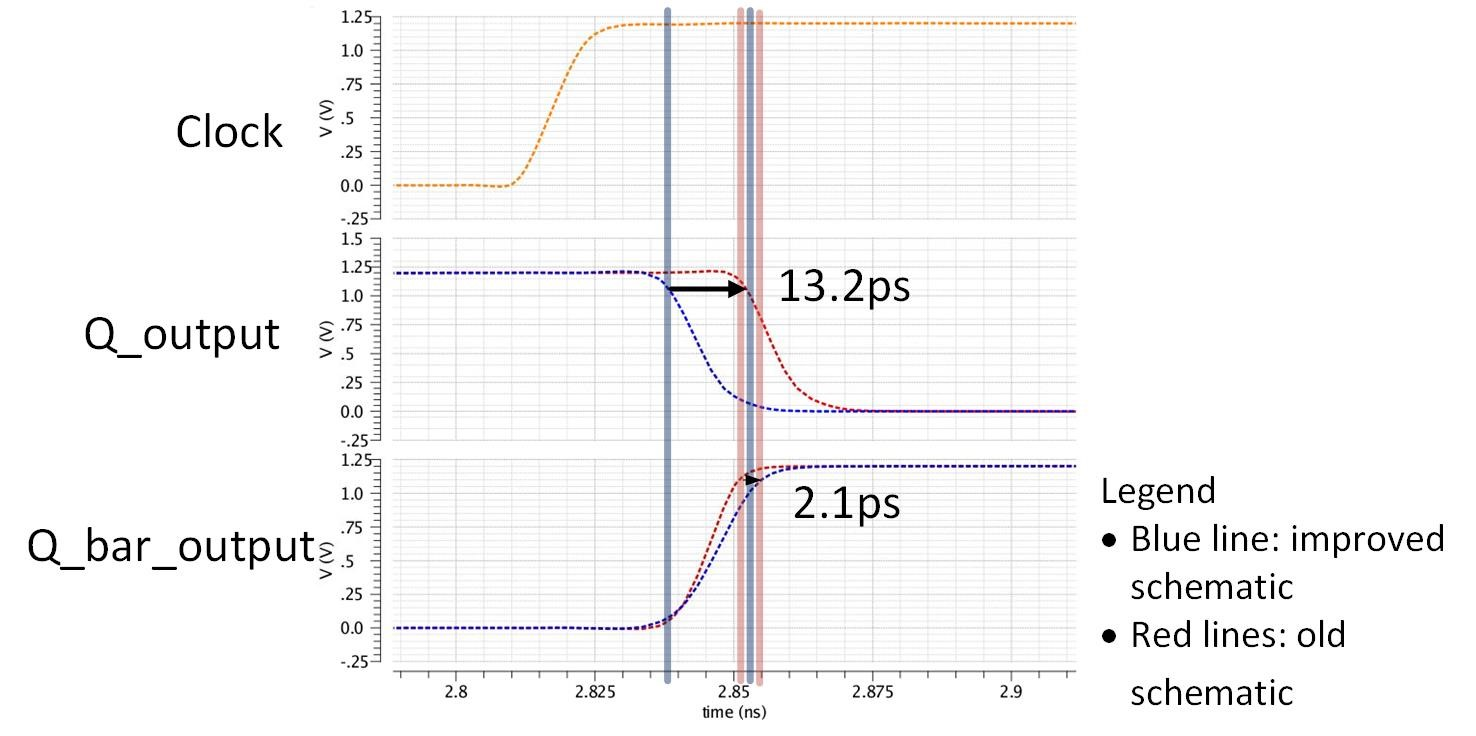
\includegraphics[width=0.5\textwidth]{Comparison_old_schematic_and_new_schematic_low.jpg}
\caption{ Comparison of the transition delay before and after improvements when the data is low.}
\label{fig:Comparison_old_schematic_and_new_schematic_low_figure}
\end{figure}

With all the transistors sizes chosen, the critical point can be measured to measure the minimum time that is needed to set the data before the clock is high. The minimal time that the data needs to be set is 40ps. The transition delay of Q and \textoverline{Q} is 29ps when the data is high. When the data is low the delay of Q is 27ps and \textoverline{Q} is 32ps. This is shown in Fig.~\ref{fig:Critical_values_flip_flop_figure}.The final sizes of transistors in the D flip-flop are listed in Appendix~\ref{sec:appendix} in Tables~\ref{Tab:D_flip-flop_transistor_sizes}.

\begin{figure}[h]
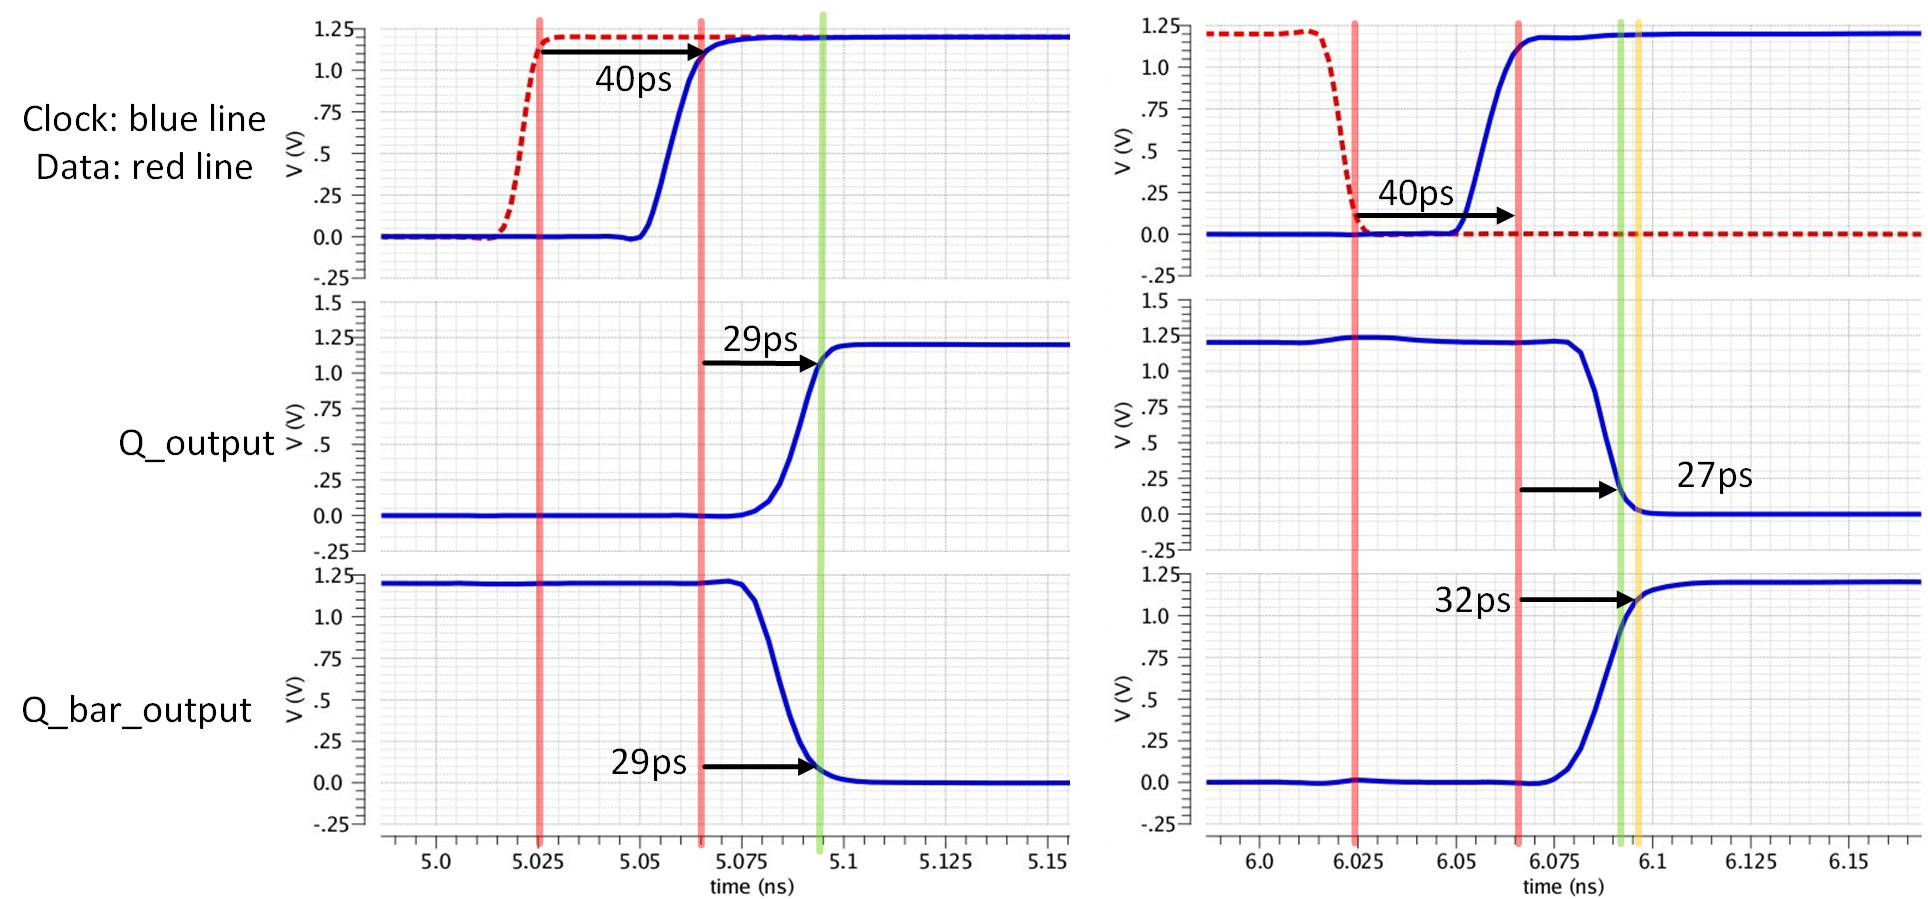
\includegraphics[width=0.5\textwidth]{Critical_values_flip_flop.jpg}
\caption{ Critical values of the settling time of the date and the delay of the transition of the output signal}
\label{fig:Critical_values_flip_flop_figure}
\end{figure}

\subsubsection{NAND and NOR gates}\label{sec:frontend}
The NAND and NOR gates mix LO signal with the data from the D flip-flop. This happens with an LO signal consisting of a 2GHz square wave.

The NAND gate has two PMOS transistors in parallel and 2 NMOS transistors in series. The schematic is shown in Appendix A, Fig.~\ref{fig:NAND_schematic_figure}. In a normal CMOS inverter the width of the PMOS transistors is 2 to 3 times larger than the NMOS transistors, because the mobility of the NMOS transistor is larger than the PMOS transistor. The size of the PMOS transistor is 50nm x 180nm (length x width). In this situation two NMOS transistors are in series. The width of the NMOS has been determined with a parameter sweep and the length is set to 50nm. The result is shown in Appendix A, Fig.~\ref{fig:NAND_nmos_sweep_figure}. The optimal value for the width is 180nm is, because it has the same fall and rise times. The size of the NMOS transistor and PMOS transistor is 50nm x 180nm (length x width).

The NOR gate has two PMOS transistors in series and 2 NMOS transistors in parallel.The schematic is shown in Appendix A, Fig.~\ref{fig:NOR_schematic_figure}. The size of the NMOS transistor is set on the smallest size of a NMOS transistor: 50nm x 90nm (length x width). The width of the PMOS transistor is determined with a parameter sweep and the length is set to 50nm. The result is shown in Appendix, Fig.~\ref{fig:NOR_pmos_sweep_figure}. The optimal value for the width is 280nm is, because it has the same fall and rise time. The size of the PMOS transistor is 50nm x 280nm (length x width).

Remark
In the simulation the load of the level shifter is increased. The NAND gates and NOR gates cannot provide the required current to drive the levels shifter, therefore a CMOS buffer is placed behind the NAND and NOR gate. The width of the PMOS transistor is set on 900nm and the NMOS transistor is set on 500nm. The results of the buffer is shown Appendix A, Fig. Fig.~\ref{fig:Results_of_NAND_NOR_with_buffer_figure}.

